\section{Análise Estatística Descritiva}
\label{sec:analise-descritiva}

Esta seção caracteriza a distribuição do número de tentativas até o sucesso nos 27 cenários executados. Como todo cenário termina em sucesso, o número de erros de um cenário é igual a esse número menos um. A variável é uma contagem (escala de razão) e, portanto, admite todas as medidas descritivas usuais \cite[Tabela 11.1, p.~154]{Wohlin2012}.

Como o estudo é de caso único e o conjunto de dados é pequeno ($n = 27$), a análise quantitativa é descritiva e exploratória, sem teste de hipótese sobre a QE-1. \citeonline[p.~99]{Wohlin2012} incluem a estatística descritiva entre as atividades de análise quantitativa em estudos de caso e alertam que conjuntos de dados quantitativos de casos únicos tendem a ser muito pequenos. Foram aplicadas medidas de tendência central e de dispersão, além de visualização gráfica \cite[Cap.~11.1, p.~153--161]{Wohlin2012}. O desvio-padrão, a variância e o coeficiente de variação usam a fórmula amostral ($n - 1$), e os quartis usam interpolação linear. O $n = 27$ refere-se a cenários; o número de tentativas com falha também é 27, o que é uma coincidência numérica decorrente de a média ser exatamente 2,0 tentativas por cenário.

\subsection{Distribuição das tentativas por cenário}
\label{subsec:distribuicao-cenario}

A Figura~\ref{fig:tentativas-por-us} mostra o número de tentativas até o sucesso de cada cenário, ordenado do que exigiu mais tentativas para o que exigiu menos. As barras de altura 1 correspondem aos cenários sem erros na primeira execução, ou seja, ao resultado da Métrica 1.9.

\begin{figure}[htb]
\centering
\caption{Tentativas até o sucesso, por cenário}
\label{fig:tentativas-por-us}
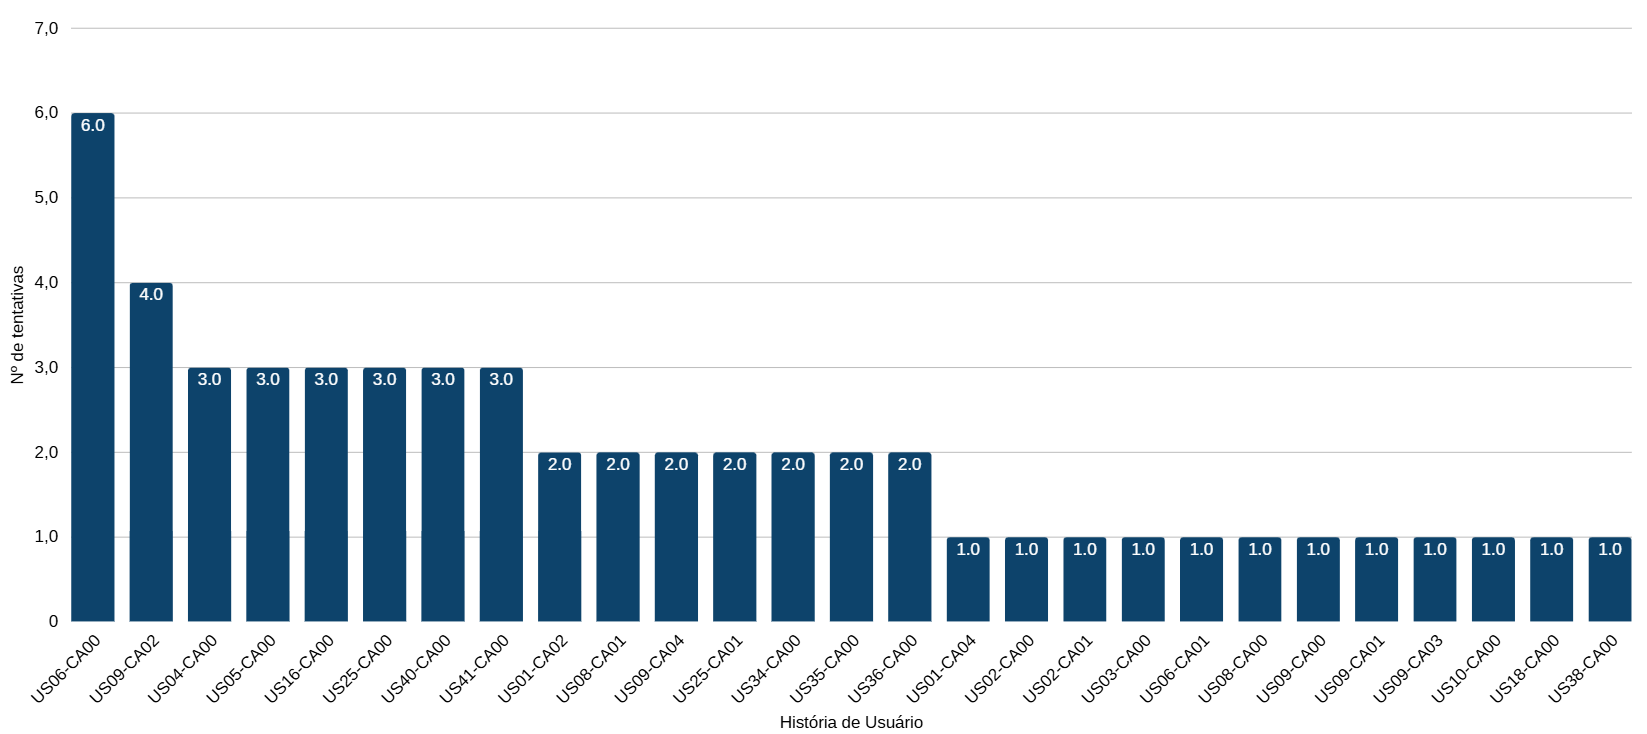
\includegraphics[width=\textwidth]{figuras/n_tentativas.png}
\legend{Fonte: Autores (2026).}
\end{figure}

Doze cenários precisaram de apenas uma tentativa, sete de duas e seis de três. Os dois casos mais extremos foram a US09-CA02, com quatro tentativas, e a US06-CA00, com seis, a única que chegou a cinco erros. A maior parte dos cenários (25 de 27) ficou, portanto, entre uma e três tentativas.

\subsection{Medidas de tendência central e de dispersão}
\label{subsec:medidas-descritivas}

A Tabela~\ref{tab:descritiva} resume a distribuição do número de tentativas até o sucesso, e a Figura~\ref{fig:boxplot} a apresenta em um \textit{box plot}.

\begin{table}[htb]
\centering
\caption{Estatística descritiva do número de tentativas até o sucesso}
\label{tab:descritiva}
\begin{tabular}{lr}
\hline
\textbf{Medida} & \textbf{Valor} \\
\hline
$n$ & 27 (cenários) \\
Média & 2,0 \\
Mediana & 2,0 \\
Moda & 1 (44,4\% dos cenários) \\
Desvio-padrão & 1,21 \\
Variância & 1,46 \\
Mínimo -- Máximo & 1 -- 6 \\
Amplitude & 5 \\
Coeficiente de variação & 60,4\% \\
Q1 -- Q3 (IQR) & 1 -- 3 (IQR = 2) \\
\hline
\end{tabular}
\legend{Fonte: Autores (2026).}
\end{table}

\begin{figure}[htb]
\centering
\caption{\textit{Box plot} do número de tentativas até o sucesso}
\label{fig:boxplot}
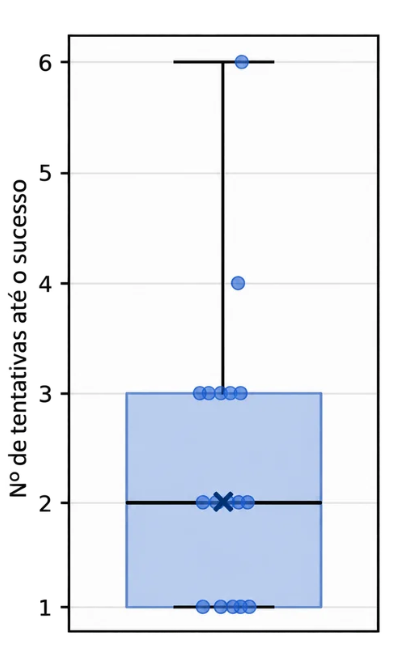
\includegraphics[width=0.42\textwidth]{figuras/boxplot.png}
\legend{Fonte: Autores (2026).}
\end{figure}

Os resultados permitem as seguintes leituras:

\begin{itemize}
    \item \textbf{Tendência central.} A mediana é de 2 tentativas e a moda é 1, que ocorre em 44,4\% dos cenários (12 de 27), exatamente os cenários sem erros na primeira execução. Em termos de erros (tentativas menos um), a mediana é 1 e a moda é 0.
    \item \textbf{Metade central dos cenários.} Os cenários entre o primeiro e o terceiro quartil precisaram de 1 a 3 tentativas (IQR = 2).
    \item \textbf{Assimetria.} A média e a mediana coincidem (2,0), mas a distribuição não é simétrica: em uma distribuição simétrica, média, mediana e moda são iguais \cite[Fig.~11.2, p.~156]{Wohlin2012}, e aqui a moda (1) difere de ambas. A assimetria está na cauda superior, que chega a 6 tentativas, enquanto o lado inferior esbarra no piso natural de uma tentativa.
    \item \textbf{Valor máximo.} O máximo (6 tentativas, US06-CA00) coincide com o limite superior do bigode (Q3 + 1,5 × IQR = 3 + 1,5 × 2 = 6) e, portanto, não é um \textit{outlier} formal pela regra adotada por \citeonline[p.~160]{Wohlin2012}. Ele está, porém, a mais de dois desvios-padrão acima da média (2,0 + 2 × 1,21 = 4,42) e é o cenário mais atípico do conjunto.
    \item \textbf{Dispersão.} O coeficiente de variação de 60,4\% indica dispersão relativa elevada, ou seja, o número de tentativas até o sucesso é bastante heterogêneo entre os cenários.
\end{itemize}

\subsection{Verificação da normalidade da distribuição}
\label{subsec:normalidade}

Como a média e a mediana coincidem, mas a moda difere delas, verificou-se se a distribuição se aproxima de uma normal. Segundo \citeonline[p.~160--161]{Wohlin2012}, o histograma dá uma primeira indicação disso, e a normalidade também pode ser testada, por exemplo, pelo teste de Shapiro-Wilk \cite[p.~183]{Wohlin2012}. A verificação importa porque técnicas paramétricas se baseiam, em geral, na suposição de normalidade \cite[p.~166]{Wohlin2012}. Como no nosso caso ela não é um teste de hipótese sobre a QE-1, o real objetivo é indicar se a média e o desvio-padrão resumem bem a variável. Foram utilizados o teste de Shapiro-Wilk e o histograma com a curva normal ajustada (Figura~\ref{fig:histograma}).

\begin{figure}[htb]
\centering
\caption{Histograma do número de tentativas até o sucesso, com a curva normal ajustada}
\label{fig:histograma}
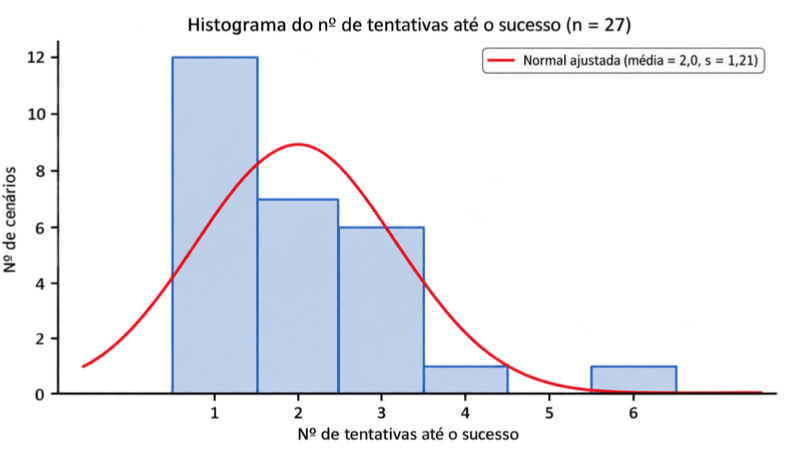
\includegraphics[width=0.75\textwidth]{figuras/histograma.png}
\legend{Fonte: Autores (2026).}
\end{figure}

Como podemos ver abaixo, o teste de Shapiro-Wilk rejeitou a normalidade ($W = 0{,}78$; $p < 0{,}001$), e a assimetria de 1,46 confirma a cauda à direita, com o histograma evidenciando um pico em uma tentativa, uma cauda longa à direita e nenhum valor abaixo de 1. A curva normal ajustada atribui probabilidade a zero tentativa ou menos, o que é impossível para essa variável. \citeonline[p.~183]{Wohlin2012} lembram que, em amostras pequenas, os testes de normalidade têm pouco poder, mas aqui a rejeição é clara. Os valores de $p$ são aproximados, pois a variável é discreta e tem muitos empates.

A distribuição não pode, portanto, ser tratada como normal, e a média e o desvio-padrão, isoladamente, resumem mal o número de tentativas. Por isso, a descrição desta seção se apoia também na mediana, nos quartis, na moda e nas frequências, que não dependem da normalidade. Isso é coerente com a opção por uma análise descritiva neste estudo de caso.

As medidas e a verificação de normalidade caracterizam a distribuição dos erros, mas não explicam por que eles ocorrem. A Seção~\ref{sec:analises-complementares} aborda as causas das falhas e as correções realizadas.
